\documentclass{article}

\usepackage{algorithmic}
\usepackage{amsmath}
\usepackage{graphicx}
\usepackage{hyperref}
\usepackage{booktabs}

\begin{document}

\title{Neural Network Handwriting Recognition}
\author{Geoffrey Ulman\\
        Midterm Exam\\
        CSI873}
\date{October 2011}
\maketitle

\tableofcontents

\section{Network Implementation}\label{Network Parameters}

The neural network used to classify the provided handwriting data set was a feed-forward network with 64 input nodes (one for each pixel in the input images), 10 output nodes (one for each digit 0 through 9), and one hidden layer. A number of different node counts for the hidden layer were tried and compared. The input and hidden layers also contained a threshold node whose output value was always fixed at \(1.0\). Each node in the hidden and output layers was implemented as a sigmoid threshold unit. Equation \ref{sigmoid1} demonstrates the calculations performed at a single node with inputs \(x_{0}\) through \(x_{n}\) and weights \(w_{0}\) through \(w_{n}\).

\begin{equation}\label{sigmoid1}
\begin{split}
net &= \sum\limits_{i=0}^n w_{i}x_{i}\\
\sigma_{net} &= \frac{1}{1+e^{-net}}
\end{split}
\end{equation}

The stochastic backpropagation algorithm was used to train the network. Simple experiments (described below) were performed to gain intuition about what training rates and momentum parameters worked well for this data set. A learning rate of \(0.15\) and a momentum of \(0.3\) were used for the final runs. Network weights were randomly initialized between \(-0.1\) and \(0.1\) before training began.

\subsection{Expected Output}

\begin{figure}\label{expected1}
\[ \begin{Bmatrix} 0.1 & 0.1 & 0.9 & 0.1 & 0.1 & 0.1 & 0.1 & 0.1 & 0.1 & 0.1 \end{Bmatrix} \]
\caption{Expected output vector for digit: 2}
\end{figure}

Values of \(0.9\) and \(0.1\) (instead of \(0.0\) and \(1.0\)) were used for the entries in the length 10 output vector for the training examples. This greatly reduced the tendancy of the weights to take on very large values during training (because the sigmoid has horizontal asymptotes near \(0.0\) and \(1.0\). Figure \ref{expected1} demonstrates the expected output vector for a \(2\) digit.

\subsection{Stopping Criteria}

A group of \(50\) training examples (five from each digit) were set aside from the \(930\) training examples to be used as a validation data set. After each iteration, the error rate was evaluated against this validation sample. The training was stopped if the error rate of the validation sample had not improved in the past (aproximately) 200,000 iterations.

\section{Data Sets}\label{Dataset}

The neural network described above was trained to classify \(8\) by \(8\) pixel handwriting samples with \(1\) bit of information per pixel. A total of \(930\) training samples and \(410\) testing samples was provided. Figure \ref{train_all} provides a visualization of each training sample and Figure \ref{test_all} provides a visualization of each testing sample.

\begin{figure}
\centering
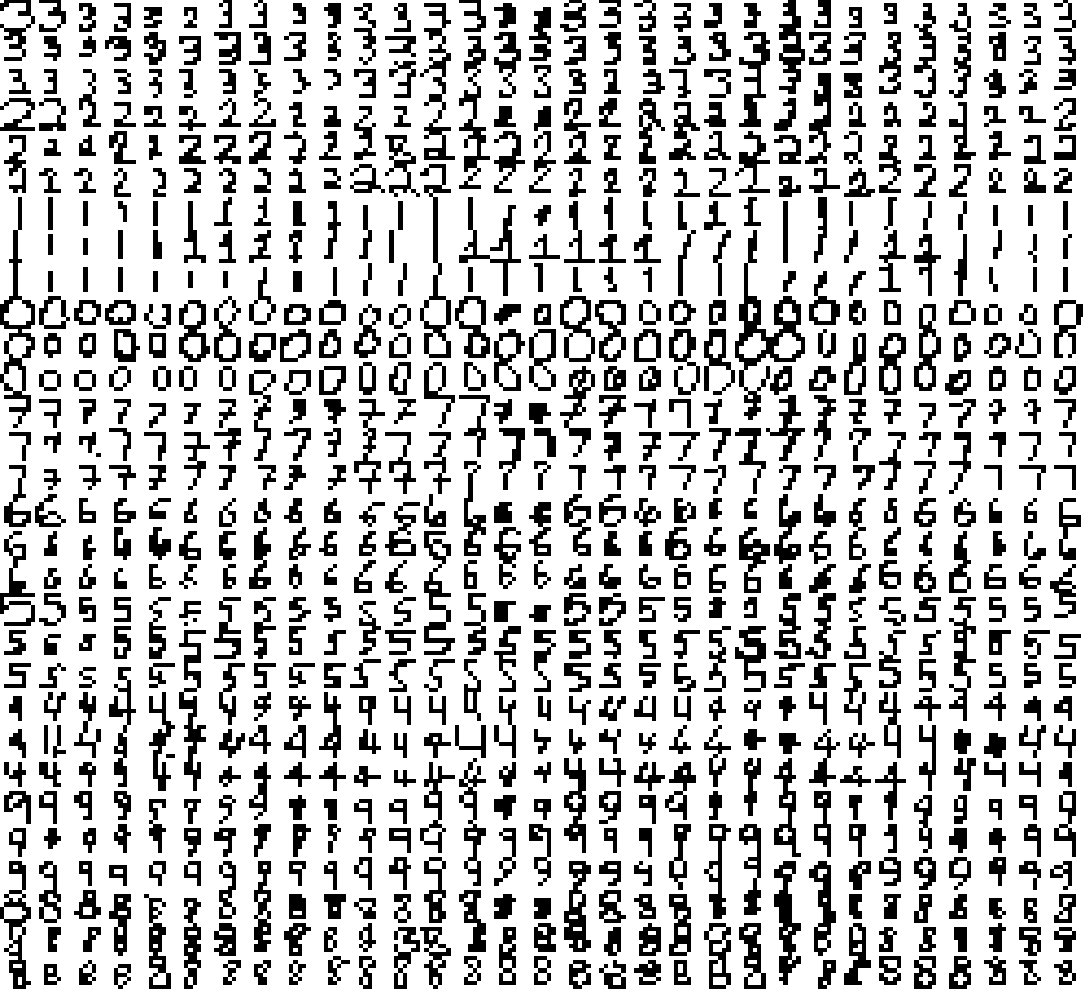
\includegraphics[width=0.85\textwidth]{data/visualization/all_training_data.png}
\caption{Handwriting samples from training data set}
\label{train_all}
\end{figure}

\begin{figure}
\centering
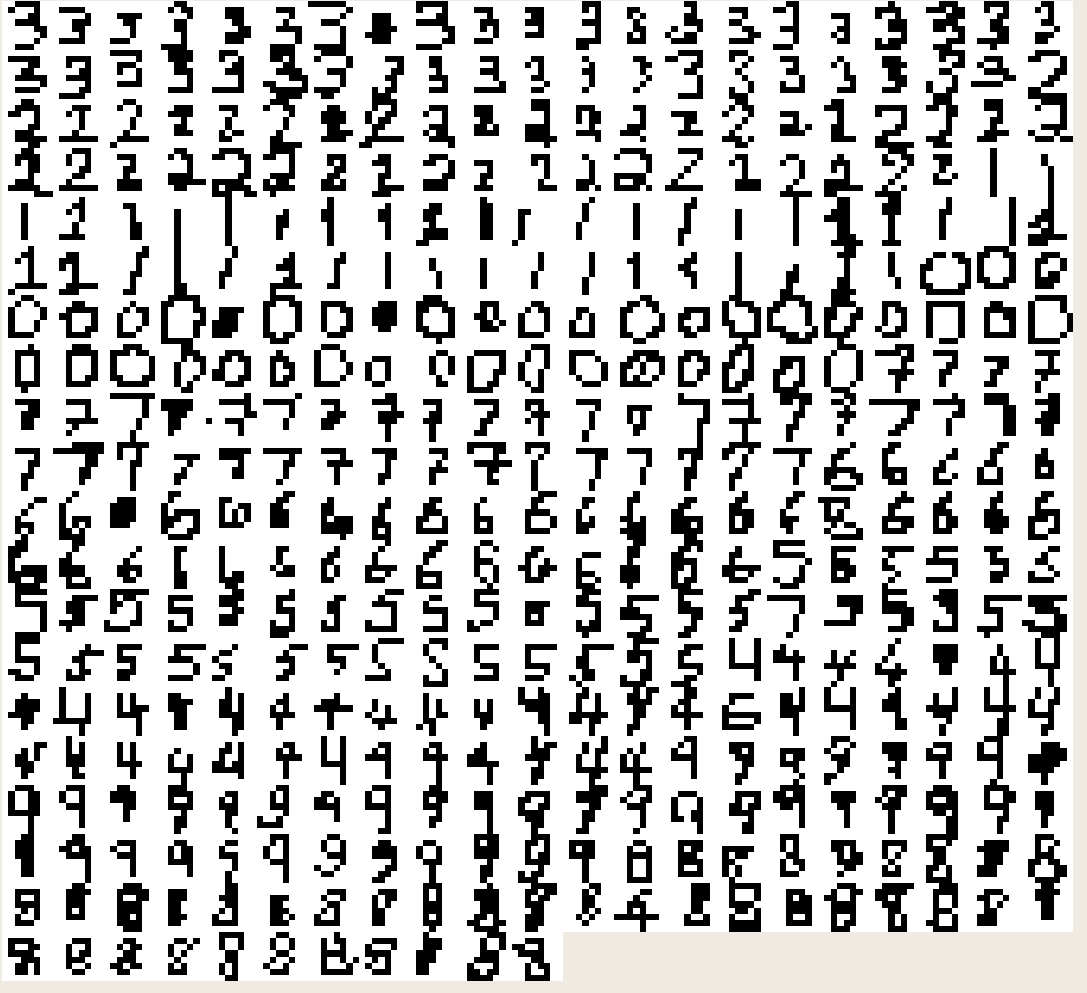
\includegraphics[width=0.85\textwidth]{data/visualization/all_testing_data.png}
\caption{Handwriting samples from test data set}
\label{test_all}
\end{figure}

\section{Software Implemenation}\label{Software Implemenation}

Java (version 1.6.0\_27) was used to implement the neural network and training algorithm. The code is available as a Subversion repository on Google Code at \url{http://code.google.com/p/csi873/}. Compiling and running the code requires the Java build tool Maven (\url{http://maven.apache.org/}). Plots were generated using the Java plotting library JFreeChart (\url{http://www.jfree.org/jfreechart/}). The Google Java general purpose Java utility library Guava (\url{http://code.google.com/p/guava-libraries/}) was also utilized for its multi-map collection data structures.

The source code is also included in the appendix and is organized with code implementing the core backpropagation algorithm and network structure up front, with less critical I/O and support code behind. Of particular interest is the Backpropagation class, which implements the stochastic backpropagation algorithm, the AbstractNet class, which handles network construction and calculation of network output, and the SigmoidNode class, which provides error, output, and weight update calculations specific to networks using a sigmoid activation function (see Equation \ref{sigmoid1}). Finnaly, the Midterm class is the main class responsible for using the components described above to load data, constructing and train a network, and output results.

Prior project work completed for CSI710 (Scientific Databases) was utilized to create the handwriting sample visualizations and confusion matrix plots. The code the visualization software is also available as a Subversion repository on Google Code at \url{http://code.google.com/p/csi701-group2/}.

\section{Results}\label{Results}

Experiments were performed with 2, 3, and 4 hidden layers as indicated by the exam instructions. In adition, out of curiosity, a network with a 10 node hidden layer was also tested. Results for each case are summarized in the following sections.

\subsection{Two Hidden Nodes}\label{hidden2}

The two hidden node network required aproximately 200,000 stochastic backpropagation algorithm iterations to train. The final error evaluated against the testing data set was \(0.720\) with a 95\% confidence interval of \((0.676 , 0.763)\). The confidence interval calculation is summarized in Equation \ref{conf2sample}.

\subsection{Confidence Interval Discussion (Question 2c)}\label{hidden2}

Table \ref{table2} summarizes the missclassification error and 95\% confidence intervals for the testing, validation, and training data sets. Although the training error confidence interval is based on more samples, and is thus tighter, the testing error confidence interval provides a more realistic estimate of the true error of the two hidden node neural network classifier as applied to unseen data. This is because the network may be overfit to the particular characteristics of the training data samples which might not be representative of the overall class of all possible input data. Therefore, the error measured using the the testing data set (which was not used to train the algorithm) provides a more realistic sense regarding how the classifier will perform on new data. 

\begin{equation}\label{conf2sample}
\begin{split}
error_{S}(h) &\pm z_{N}\sqrt{\frac{error_{S}(h)(1-error_{S}(h))}{n}} \\
0.72 &\pm 1.96\sqrt{\frac{(0.72)(1-0.72)}{410}} 
\end{split}
\end{equation}

\begin{table}
\caption{Missclassification Error for 2 Hidden Node Network}
\begin{center}
\begin{tabular}{llcc}
\toprule
Data Set & Error & \multicolumn{2}{c}{95\% Confidence Interval} \\
\cmidrule(r){3-4}
& & Lower Bound & Upper Bound \\
\midrule
Testing       & 0.720 &  0.676 & 0.763  \\
Validation    & 0.760 &  0.642 & 0.878  \\
Training      & 0.702 &  0.672 & 0.732  \\
\bottomrule
\end{tabular}
\label{table2}
\end{center}
\end{table}

Figure \ref{error2} summarizes the training process of the two hidden node network by plotting the evolution of the training and validation errors during training. Figure \ref{weight2} plots the evolution of the weights for the output node associated with the digit ``0''.

\begin{figure}
\centering
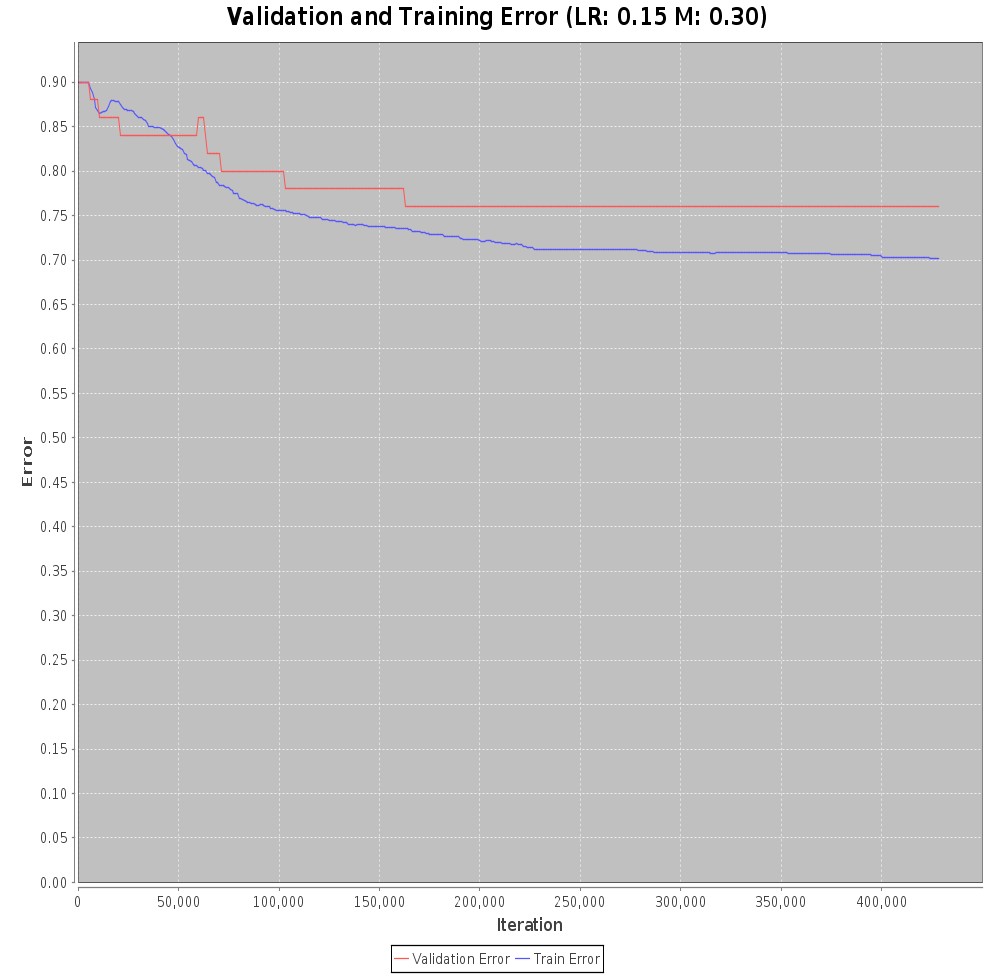
\includegraphics[width=0.7\textwidth]{data/final/2_hidden_node_error.png}
\caption{Missclassification Error for 2 Hidden Node Network by Iteration}
\label{error2}
\end{figure}

\begin{figure}
\centering
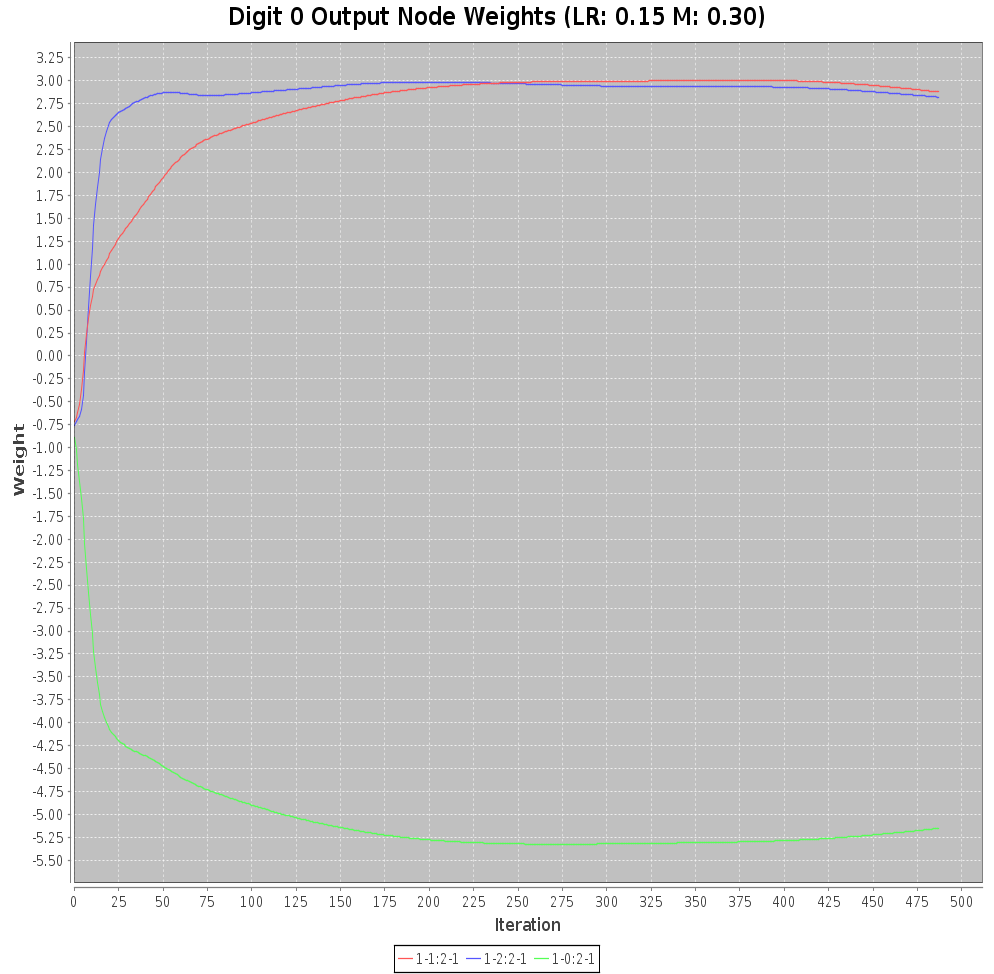
\includegraphics[width=0.7\textwidth]{data/final/2_hidden_node_0weight.png}
\caption{Output Node 0 Input Weights for 2 Hidden Node Network by Iteration}
\label{weight2}
\end{figure}

Figures \ref{testconfusion2} and \ref{trainconfusion2} summarize the error rate of the trained network against the testing and training data sets on a digit-by-digit basis. Each box represents the number of handwriting samples which were classified as the digit in the column header but were actually instances of the digit in the row header. Thus, correct classifications are listed along the diagonal of the confusion matrix. The boxes are color coded on a blue to red scale according to the number of handwriting samples falling in the box. Note: because rows indicate the true digit represented by the handwriting samples, the values in each row add up to 41 in the testing data case and 93 in the training data case.

It is clear from Figures \ref{testconfusion2} and \ref{trainconfusion2} (as well as the errors reported in Table \ref{table2}) that two hidden nodes does not provide sufficient degrees of freedom to allow the neural network to distinguish between all ten characters. The resulting decision surfaces are simply insufficiently complex. In this particular case, the network classifies the digits 0 and 7 with some accuracy and classifies almost all other training examples as either 8 or 9.

\begin{figure}
\centering
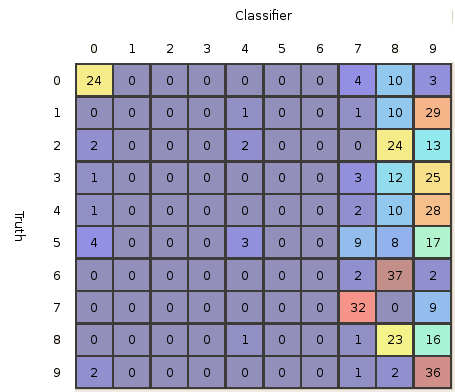
\includegraphics[width=0.7\textwidth]{data/final/2_test_confusion.png}
\caption{Confusion Matrix for Testing Data Set for 2 Hidden Node Network}
\label{testconfusion2}
\end{figure}

\begin{figure}
\centering
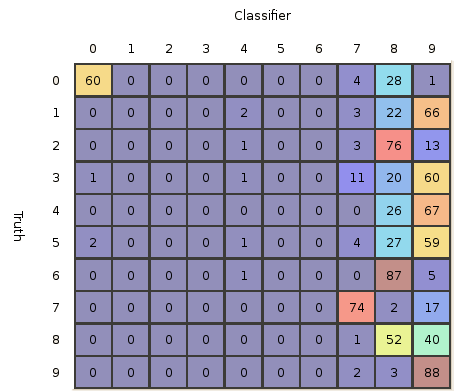
\includegraphics[width=0.7\textwidth]{data/final/2_train_confusion.png}
\caption{Confusion Matrix for Training Data Set for 2 Hidden Node Network}
\label{trainconfusion2}
\end{figure}

\subsection{Three Hidden Nodes}\label{hidden3}

Missclassification error rate for testing data with three hidden nodes improved slightly to \(0.685\) with a 95\% confidence interval of \((0.640 , 0.730)\). Table \ref{table3} summarizes the missclassification error and 95\% confidence intervals for the testing, validation, and training data sets.

\begin{table}
\caption{Missclassification Error for 3 Hidden Node Network}
\begin{center}
\begin{tabular}{llcc}
\toprule
Data Set & Error & \multicolumn{2}{c}{95\% Confidence Interval} \\
\cmidrule(r){3-4}
& & Lower Bound & Upper Bound \\
\midrule
Testing       & 0.685 &  0.640 & 0.730  \\
Validation    & 0.660 &  0.529 & 0.791  \\
Training      & 0.588 &  0.555 & 0.620  \\
\bottomrule
\end{tabular}
\label{table3}
\end{center}
\end{table}

\begin{figure}
\centering
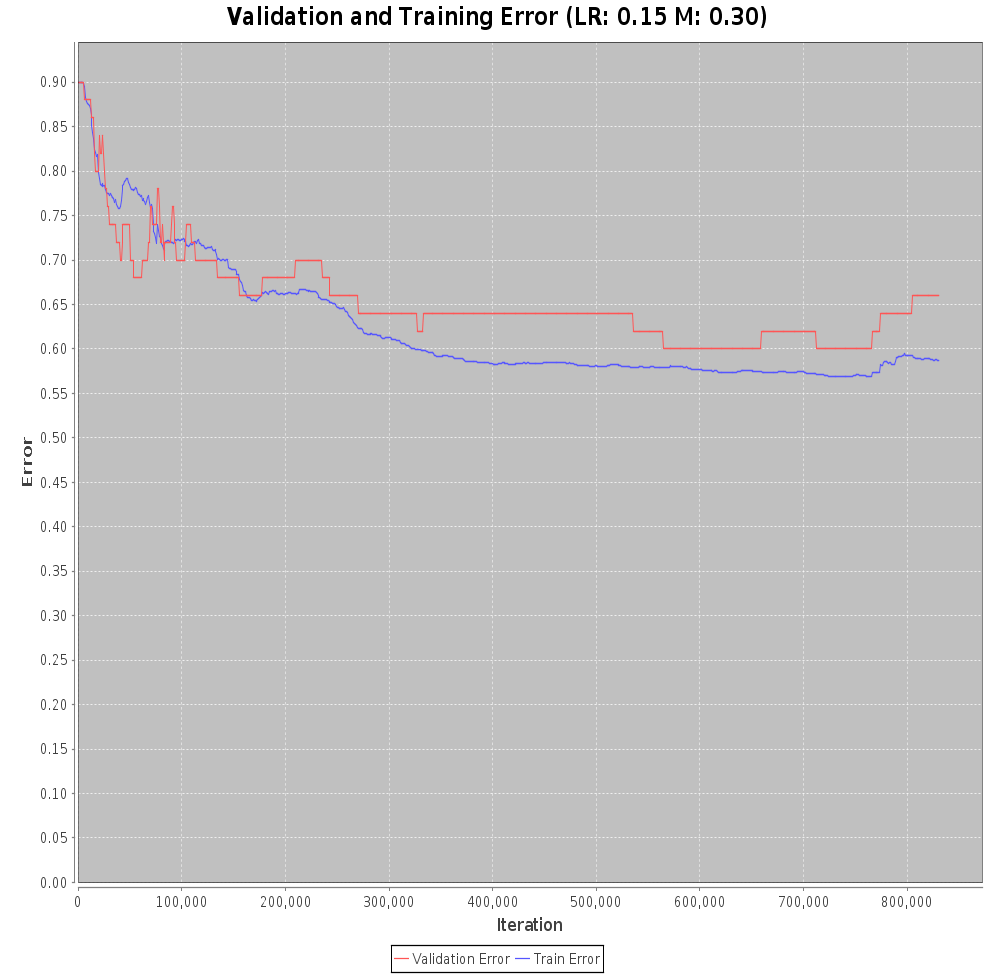
\includegraphics[width=0.7\textwidth]{data/final/3_hidden_node_error.png}
\caption{Missclassification Error for 3 Hidden Node Network by Iteration}
\label{error3}
\end{figure}

\begin{figure}
\centering
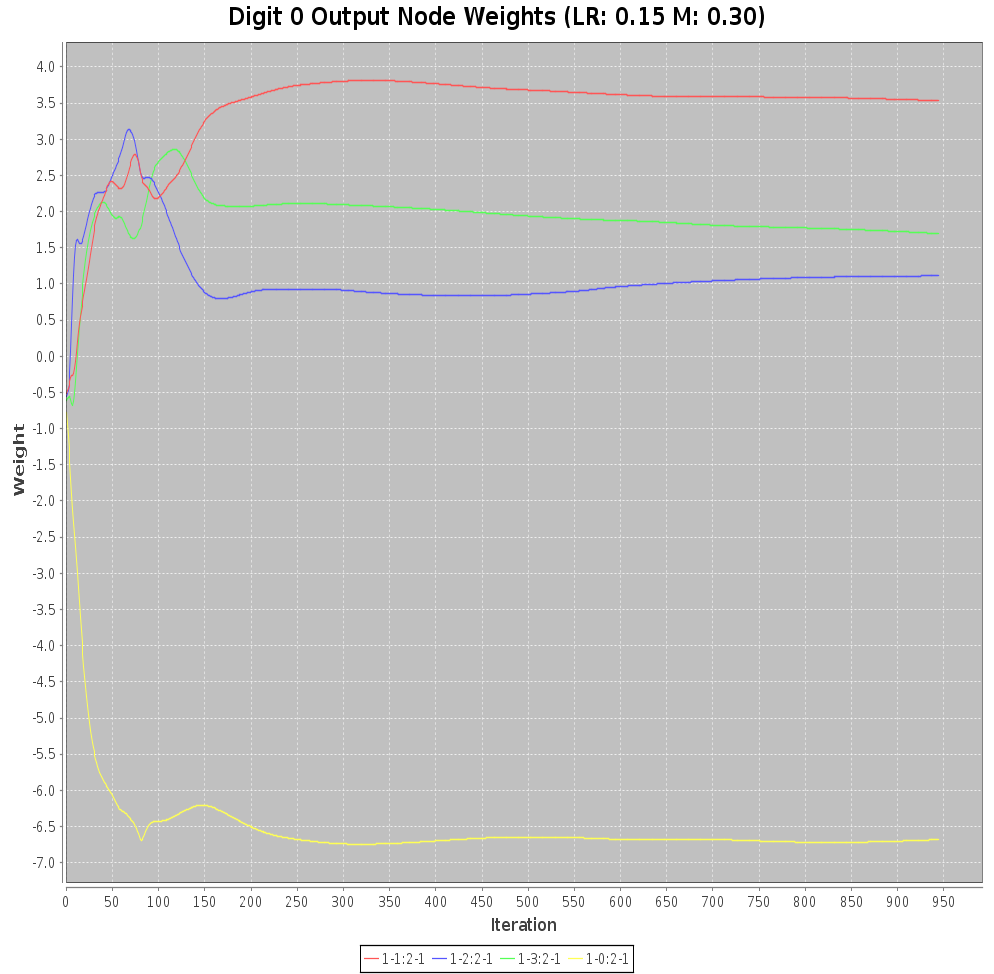
\includegraphics[width=0.7\textwidth]{data/final/3_hidden_node_0weight.png}
\caption{Output Node 0 Input Weights for 3 Hidden Node Network by Iteration}
\label{weight3}
\end{figure}

As indicated by Figure \ref{error3}, the three hidden node network took approximately 800,000 iterations to train, almsot four times longer than the two hidden node network. However, as indicated by Figure \ref{weight3}, the weights for at least some of the output nodes stabilized much earlier than that. Note that the x-axis in Figure \ref{weight3} is measured in (approximately) 1000s of iterations.

\begin{figure}
\centering
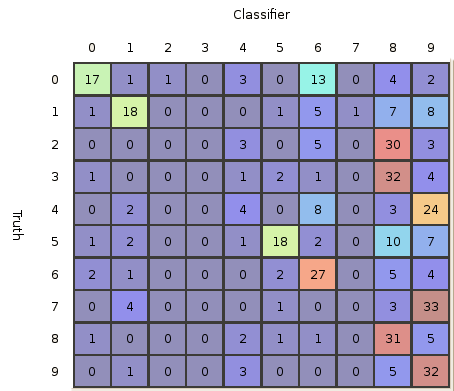
\includegraphics[width=0.7\textwidth]{data/final/3_test_confusion.png}
\caption{Confusion Matrix for Testing Data Set for 3 Hidden Node Network}
\label{testconfusion3}
\end{figure}

\begin{figure}
\centering
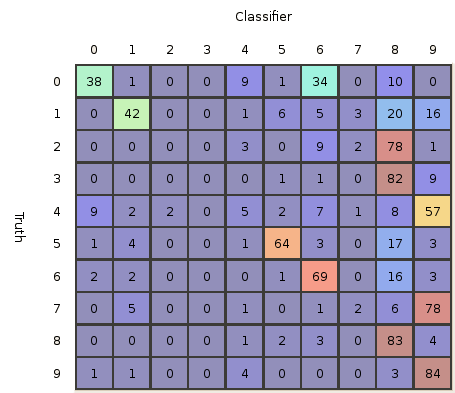
\includegraphics[width=0.7\textwidth]{data/final/3_train_confusion.png}
\caption{Confusion Matrix for Training Data Set for 3 Hidden Node Network}
\label{trainconfusion3}
\end{figure}

However, the confusion matrix in Figures \ref{testconfusion3} and \ref{trainconfusion3} make it clear that the decision surface is still not complex enough to differentiate between ten output digits with only three hidden nodes. Classification performance is now reasonable for digits ``0'', ``1'', ``5'', and ``6''. However the remainder of the handwriting samples are classified as ``8'' and ``9'' with almost no samples classified as ``2'', ``3'', ``4'', or ``7''. This indicates that more hidden nodes may yet improve performance. 

\subsection{Four Hidden Nodes}\label{hidden4}

With four hidden nodes, the missclassification error rate for the testing data set finally falls to \(0.463\) with a 95\% confidence interval of \((0.415 , 0.512)\). The confusion matrices in Figures \ref{testconfusion4} and \ref{trainconfusion4} also indicate much better performance. There are high numbers of correct classifications spread over almost all digits. The noteable exception being the digit ``4'' which is never classified correctly and is very frequently classified incorrectly as a ``9''. Given the similarity in structure between the digits ``9'' and ``4'' it is simultaneously quite striking and quite intuitive that the network would lump these two digits together.

\begin{table}
\caption{Missclassification Error for 4 Hidden Node Network}
\begin{center}
\begin{tabular}{llcc}
\toprule
Data Set & Error & \multicolumn{2}{c}{95\% Confidence Interval} \\
\cmidrule(r){3-4}
& & Lower Bound & Upper Bound \\
\midrule
Testing       & 0.463 &  0.415 & 0.512  \\
Validation    & 0.440 &  0.302 & 0.578  \\
Training      & 0.345 &  0.314 & 0.377  \\
\bottomrule
\end{tabular}
\label{table4}
\end{center}
\end{table}

\begin{figure}
\centering
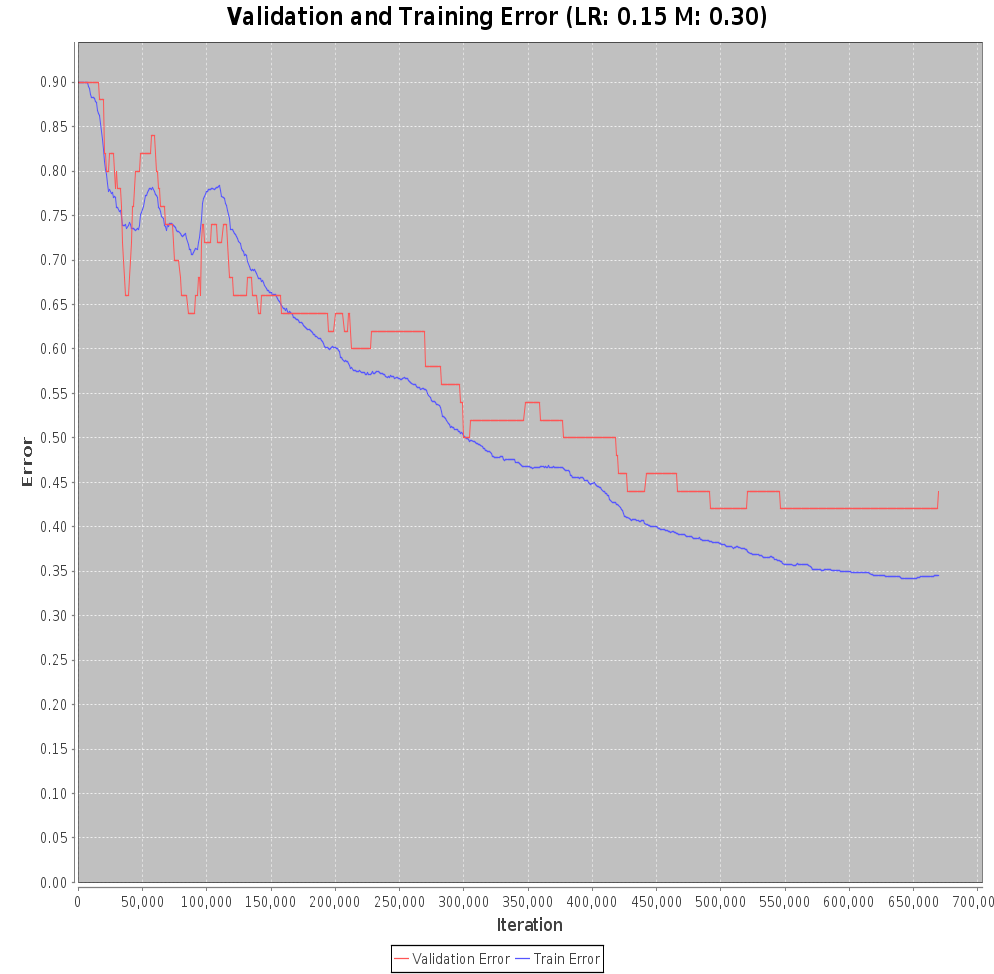
\includegraphics[width=0.7\textwidth]{data/final/4_hidden_node_error.png}
\caption{Missclassification Error for 4 Hidden Node Network by Iteration}
\label{error4}
\end{figure}

\begin{figure}
\centering
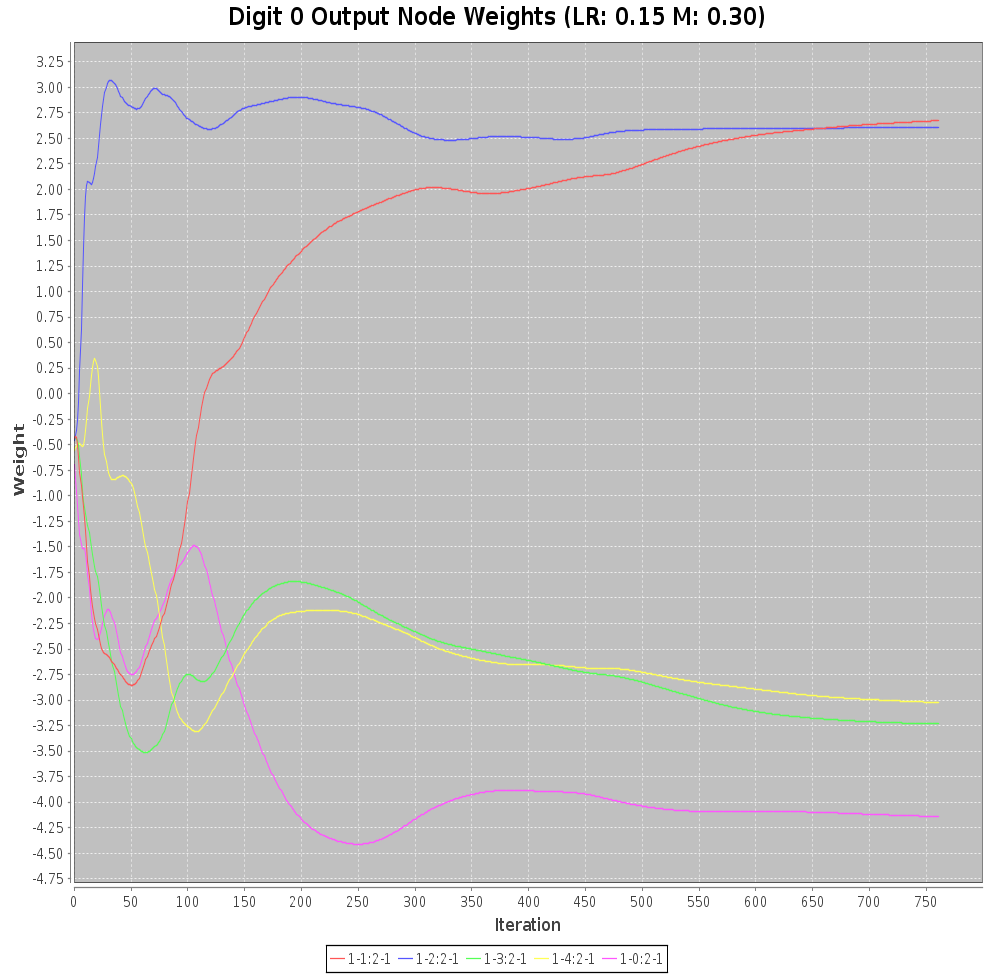
\includegraphics[width=0.7\textwidth]{data/final/4_hidden_node_0weight.png}
\caption{Output Node 0 Input Weights for 4 Hidden Node Network by Iteration}
\label{weight4}
\end{figure}

\begin{figure}
\centering
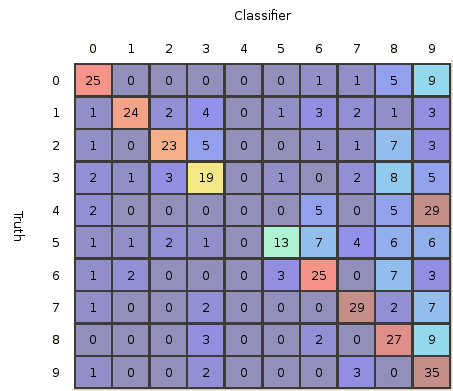
\includegraphics[width=0.7\textwidth]{data/final/4_test_confusion.png}
\caption{Confusion Matrix for Testing Data Set for 4 Hidden Node Network}
\label{testconfusion4}
\end{figure}

\begin{figure}
\centering
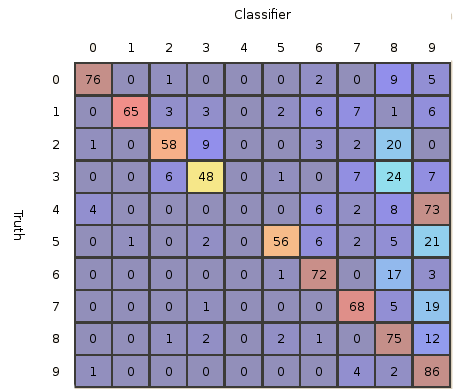
\includegraphics[width=0.7\textwidth]{data/final/4_train_confusion.png}
\caption{Confusion Matrix for Training Data Set for 4 Hidden Node Network}
\label{trainconfusion4}
\end{figure}

\subsection{Ten Hidden Nodes}\label{hidden10}

Because the results in Figures \ref{testconfusion4} and \ref{trainconfusion4} for the four hidden node network indicated that the network still had an insufficiently complicated decision boundary to differentiate between all ten digits, I performed an additional experiment with ten hidden nodes. This resulted in a significantly improved testing error rate of \(0.385\) with a 95\% confidence interval of \((0.338 , 0.432)\). Further, as indicated in Figures \ref{testconfusion10} and \ref{trainconfusion10}, the neural network is finally able to correctly classify the majority of handwriting instances for all of the ten digits.

\begin{table}
\caption{Missclassification Error for 10 Hidden Node Network}
\begin{center}
\begin{tabular}{llcc}
\toprule
Data Set & Error & \multicolumn{2}{c}{95\% Confidence Interval} \\
\cmidrule(r){3-4}
& & Lower Bound & Upper Bound \\
\midrule
Testing       & 0.385 &  0.338 & 0.432  \\
Validation    & 0.380 &  0.245 & 0.515  \\
Training      & 0.110 &  0.090 & 0.131  \\
\bottomrule
\end{tabular}
\label{table10}
\end{center}
\end{table}

\begin{figure}
\centering
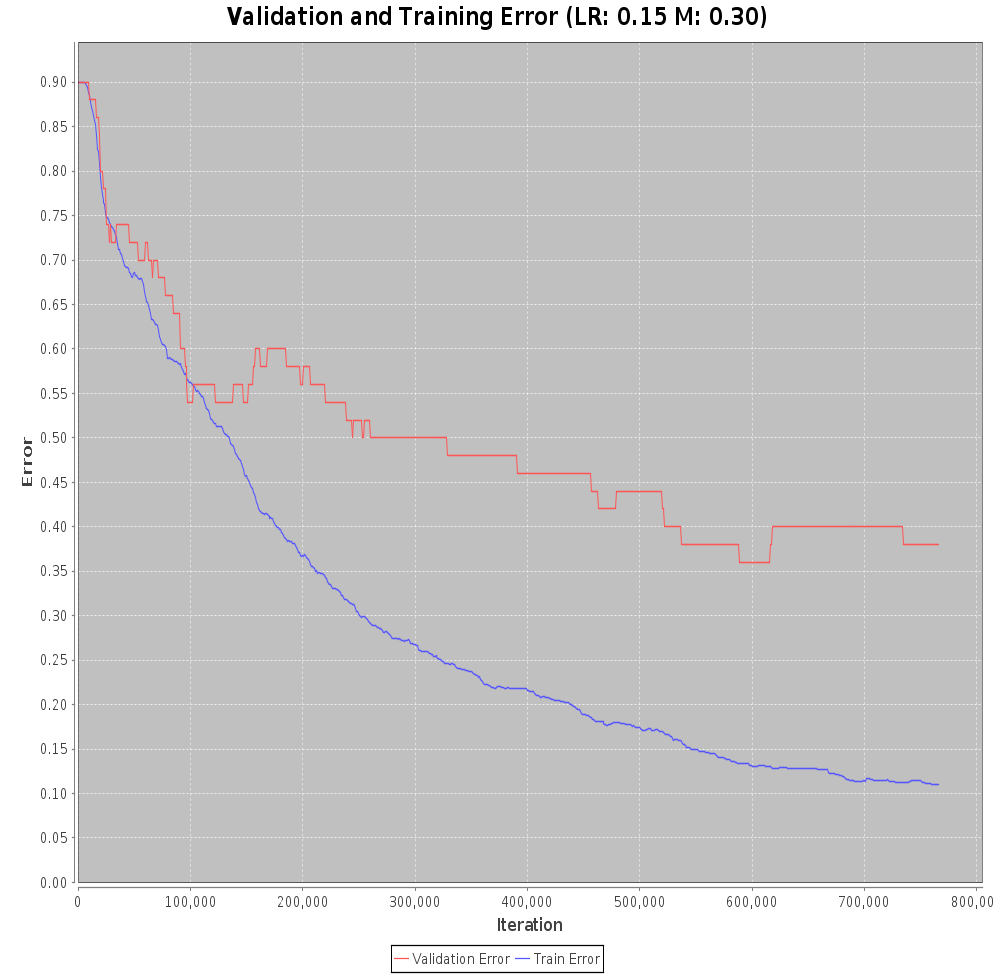
\includegraphics[width=0.7\textwidth]{data/final/10_hidden_nodes_error.png}
\caption{Missclassification Error for 10 Hidden Node Network by Iteration}
\label{error10}
\end{figure}

\begin{figure}
\centering
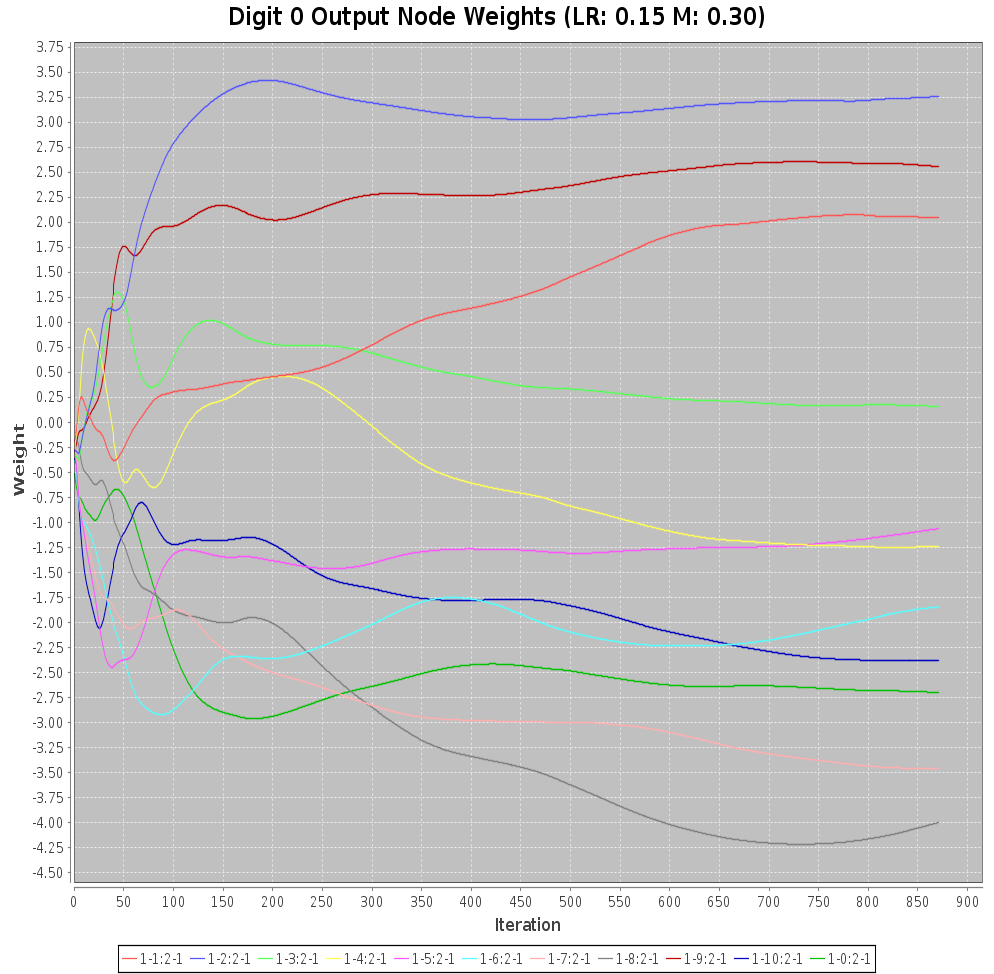
\includegraphics[width=0.7\textwidth]{data/final/10_hidden_nodes.png}
\caption{Output Node 0 Input Weights for 10 Hidden Node Network by Iteration}
\label{weight10}
\end{figure}

\begin{figure}
\centering
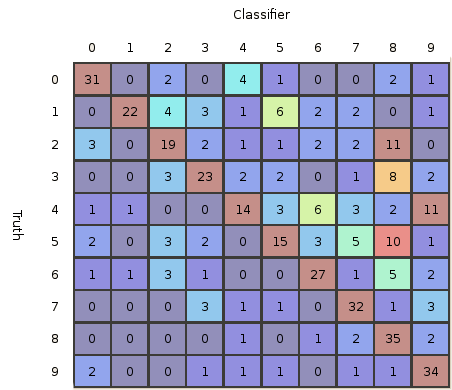
\includegraphics[width=0.7\textwidth]{data/final/10_test_confusion.png}
\caption{Confusion Matrix for Testing Data Set for 10 Hidden Node Network}
\label{testconfusion10}
\end{figure}

\begin{figure}
\centering
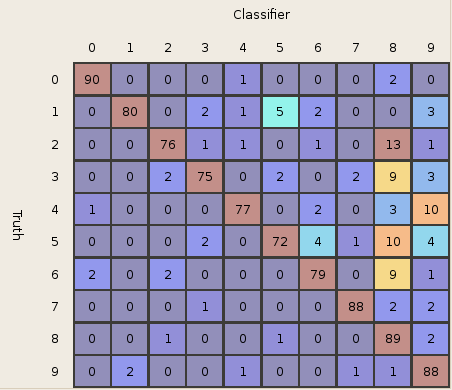
\includegraphics[width=0.7\textwidth]{data/final/10_train_confusion.png}
\caption{Confusion Matrix for Training Data Set for 10 Hidden Node Network}
\label{trainconfusion10}
\end{figure}

\begin{thebibliography}{9}

\bibitem{cpl}
  Tom M. Mitchell,
  \emph{Machine Learning},
  WCB McGraw-Hill, Boston,
  1997.

\end{thebibliography}

\end{document}
